\documentclass[
		11pt,
		a4paper,
		toc=listof, %% Abbildungs- und Tabellenverzeichnis mit ins Inhaltsverzeichnis
		bibliography=totoc %% Quellenverzeichnis mit ins Inhaltsverzeichnis
		]{scrreprt}	 %% KOMA Script

% HTWG
\usepackage{graphicx}
\usepackage{a4}
\usepackage{german}

% Eigene
\usepackage[utf8]{inputenc} %% Umlaute
\usepackage[printonlyused]{acronym} %% Abkuerzungsverzeichnis (nur verwendete)
\usepackage{todonotes} %% TODOs moeglich mit \todo{}
\usepackage{booktabs} %% Tabellen
\usepackage{amsmath} %% Formeln
\usepackage{listings} %% Codebeispiele
\usepackage{subfigure} %% Mehrere Bilder nebeneinander
\usepackage{hyperref} %% referenzen innerhalb und außerhalb des Dokumentes
\usepackage{url}
\usepackage{wrapfig}

% Eigenes Design
%TODO loeschen wenn default HTWG Design (was es nicht wirklich gibt) gewuuenscht ist
\usepackage[bottom=3cm]{geometry}
\usepackage{setspace}
\onehalfspacing


\definecolor{Gray}{rgb}{.9,.9,.9}
\definecolor{Comment}{rgb}{.40,.40,.40}
\definecolor{Blue}{rgb}{.52, .152, .219}
\definecolor{Green}{rgb}{.39, .174, .96}
\definecolor{DeepBlue}{rgb}{.44, .62, .80}

\lstdefinelanguage{JavaScript} {
	morekeywords={
		break,const,continue,delete,do,while,export,for,in,function,
		if,else,import,in,instanceOf,label,let,new,return,switch,this,
		throw,try,catch,typeof,var,void,with,yield
	},
	sensitive=false,
	morecomment=[l]{//},
	morecomment=[s]{/*}{*/},
	morestring=[b]",
	morestring=[d]'
}

\lstset{
	frame=tb,
	framesep=5pt,
	basicstyle=\footnotesize\ttfamily,
	showstringspaces=false,
	keywordstyle=\ttfamily\bfseries\color{DeepBlue},
	identifierstyle=\ttfamily,
	stringstyle=\ttfamily\color{Green},
	commentstyle=\color{Comment},
	rulecolor=\color{Gray},
	xleftmargin=5pt,
	xrightmargin=5pt,
	belowskip=\bigskipamount,
	numbers=left,
  stepnumber=1,
  firstnumber=1,
  numberfirstline=true,
	numberstyle=\normalfont\tiny\color{Comment}
}




% KOMA script anpassungen
%TODO entfernen wenn kein KOMA Script gewuenscht
\usepackage{scrhack}

%%%%%%%% Codebeispiele
\usepackage{color}
\usepackage{xcolor}
\usepackage{listings}
\usepackage{caption}

\setcounter{tocdepth}{2}  %% Uebreschriften bis subsectionw ins Inhaltsverzeichnis
\setcounter{secnumdepth}{3}  %% Nummerierung bis subsection


%%% Codebeispiele - Style
\DeclareCaptionFont{white}{\color{white}}
\DeclareCaptionFormat{listing}{\colorbox{gray}{\parbox{\textwidth}{#1#2#3}}}
\captionsetup[lstlisting]{format=listing,labelfont=white,textfont=white}

% Entfernt Kapitel Ueberschrift
% Bsp.
% 	ALT:
%       Kapitel 1
%       Einführung
%
% 	NEU:
% 		1 Einführung
%
\renewcommand*\chapterheadstartvskip{\vspace{-\topskip}}
\newcommand{\thema}{Design und Implementierung einer komponentenbasierten Cross-Platform Frontend Architektur mit Angular2, Ionic2 und Electron in Typescript}
\newcommand{\schlagworte}{Cross-Platform, Frontend Architektur, Angular2, Ionic2, Electron, Hybrid, Typescript}
\newcommand{\zusammenfassung}{Als praktischer Teil der Arbeit soll eine Frontend Architektur für ein Monitoring System für Microservices konzipiert und implementiert werden, um
mit nahezu einer Codebasis Endprodukte für Web, Desktop und Mobile zu erhalten.
Anhand der praktischen Arbeit sollen Chancen und Risiken von Web Technologien hinsichtlich Cross Plattform Entwicklungen aufgezeigt und evaluiert sowie mögliche Einschränkungen
erläutert werden. Web Komponenten sind dabei von zentraler Bedeutung. Die Applikation soll komponentenbasiert entwickelt werden, um Elemente lückenlos für genannte Plattformen wieder
verwenden zu können. Speziell soll geprüft werden, wie weit sich Komponenten, durch die Verwendung von Typescript, voneinander abstrahieren und bezüglich der Applikationsarchitektur
strukturieren lassen. Mithilfe der Frameworks Angular 2 und Ionic, welches ebenfalls auf Angular 2 aufbaut, sollen Plattformen für Web sowie iOS und Android entwickelt werden.
Zusätzlich soll mittels Electron Framework eine Plattform für native Desktop Applikation für MacOS und Windows geschaffen werden.}
\newcommand{\ausgabedatum}{15.05.2016}
\newcommand{\abgabedatum}{15.09.2016}
\newcommand{\autor}{Michael Knoch}
\newcommand{\autorStrasse}{Bücklestr. 82}
\newcommand{\autorPLZ}{78467}
\newcommand{\autorOrt}{Konstanz}
\newcommand{\autorGeburtsort}{Villingen-Schwenningen}
\newcommand{\autorGeburtsdatum}{06.06.1992}
\newcommand{\prueferA}{Prof. Dr. Marko Boger}
\newcommand{\prueferB}{Prof. Dr. Markus Eiglsperger}
\newcommand{\firma}{HTWG}
\newcommand{\studiengang}{Software-Engineering}
\newcommand{\projectname}{MIA}



\begin{document}
%% Nummerierung aus
\pagenumbering{gobble}

% HTWG Tempaltes fuer Titelseite etc.
\begin{titlepage}

\vspace*{-3.5cm}

\begin{flushleft}
\hspace*{-1cm} 
\includegraphics[width=15.7cm]{htwg/htwg-logo}
\end{flushleft}

\vspace{2.5cm}

\begin{center}
	\LARGE{
		\textbf{\thema} \\[3cm]
	}
	\Large{
		\textbf{\autor}} \\[3.5cm]
	\large{
		\textbf{Konstanz, \abgabedatum} \\[2.3cm]
	}

	\Huge{
		\textbf{{BACHELORARBEIT}}
	}
\end{center}

\end{titlepage}

\thispagestyle{empty}
{
\setlength{\parskip}{0.5cm}
        \begin{center}
        \textbf{\huge BACHELORARBEIT}

        \textbf{zur Erlangung des akademischen Grades}

        \textbf{\Large Bachelor of Science (B. Sc.)}

        \textbf{an der}

        \textsf{\huge Hochschule Konstanz}\\
        {\small Technik, Wirtschaft und Gestaltung}

        \textsf{\Large Fakult"at Informatik} \\
        Studiengang \studiengang
        \end{center}
}
\begin{center}

\vspace*{2cm}

\begin{tabular}{p{3cm}p{10cm}}
Thema: & \textbf{\large \thema} \\[15ex]
Bachelorkandidat: & \autor, \autorStrasse, \autorPLZ{}  \autorOrt{} \\[15ex]
1. Pr"ufer: & \prueferA \\
2. Pr"ufer: & \prueferB \\[25ex]
Ausgabedatum: & \ausgabedatum \\
Abgabedatum: & \abgabedatum \\
\end{tabular}
\end{center}
\begin{center}
{\Large \textbf{Zusammenfassung (Abstract)}}
\end{center}

\bigskip

\begin{center}
	\begin{tabular}{p{2.8cm}p{10cm}}
		Thema: & \thema \\
		 & \\
		Bachelorkandidat: & \autor \\
		 & \\
		Firma: & \firma \\
		 & \\
		Betreuer: & \prueferA  \\[.5ex]
		 &  \prueferB \\
		 & \\
		Abgabedatum: & \abgabedatum \\
		 & \\
		Schlagworte: & \schlagworte \\
		 & \\
	\end{tabular}
\end{center}

\bigskip

\noindent
\zusammenfassung

\pagenumbering{Roman}
\chapter*{Ehrenw"ortliche Erkl"arung}
\addcontentsline{toc}{chapter}{Ehrenw"ortliche Erkl"arung}

Hiermit erkl"are ich
\textit{\autor, geboren am \autorGeburtsdatum{} in \autorGeburtsort{}}, dass ich\\

\begin{tabular}{lp{12cm}}
(1) & meine Bachelorarbeit mit dem Titel \\[1em]
& \textbf{\thema} \\[1em]
& bei der \firma\ unter Anleitung von \prueferA\ selbst"andig und ohne fremde Hilfe angefertigt und keine anderen als die angef"uhrten Hilfen benutzt habe;\\[1em]
(2) & die "Ubernahme w"ortlicher Zitate, von Tabellen, Zeichnungen, Bildern und
Programmen aus der Literatur oder anderen Quellen (Internet) sowie die Verwendung
der Gedanken anderer Autoren an den entsprechenden Stellen innerhalb der Arbeit
gekennzeichnet habe.\\
\end{tabular}

\vspace*{1cm}

\noindent
Ich bin mir bewusst, dass eine falsche Erkl"arung rechtliche Folgen haben wird.\\

\vspace*{3cm}

\noindent
Konstanz, \abgabedatum \hfill \begin{tabular}{c} \\ \\ \rule{5cm}{1pt} \\ (Unterschrift)\end{tabular}


\tableofcontents

%!TEX root = thesis.tex

\chapter*{Abkürzungsverzeichnis}
\addcontentsline{toc}{chapter}{Abkürzungsverzeichnis}

\begin{acronym}
 \acro{UI} {User Interface}
 \acro{SDK} {Software Development Kit}
 \acro{DI} {Dependency Injection}
  \acro{OO} {Objektorientierung}
  \acro{DOM} {Document Object Model}
  \acro{JSON} {JavaScript Object Notation}
  \acro{IPA} {iOS App Store Package}
  \acro{APK} {Android application package}
  \acro{CLI} {Command Line Interface}
  \acro{APN} {Apple Push Notification}
  \acro{GCM} {Google Cloud Messaging}
  \acro{API} {Application Programming Interface}
  \acro{HTML} {Hypertext Markup Language}
  \acro{CSS} {Cascading Style Sheets}
  \acro{NPM} {Node Package Manager}
  \acro{CI} {Corporate Identity}
  \acro{MVC} {Model View Controller}
  \acro{AWS} {Amazon Web Services}
  \acro{SASS} {Syntactically Awesome Stylesheets}
\end{acronym}


%% Starte Paginierung
\cleardoublepage
\pagenumbering{arabic}

%!TEX root = ../thesis.tex

\chapter{Einführung}
\label{chap:introduction}

Bei der Planung von Softwareprojekten ist die Frage der Zielplattform meist eine der ersten und bedeutensten Fragen,
die gelöst werden muss. Eine Entscheidung darüber, welche Geräte und Betriebsysteme eine Applikation erreichen soll,
beeinflusst nicht nur nachhaltig die Zielgruppe der Anwender, sie definiert darüber hinaus wichtige Grundvoraussetzungen der Entwicklung hinsichtlich Entwicklungsumgebung, Frameworks und Tools die überhaupt genutzt werden können.

Aufgrund der umfangreichen Hersteller- und Gerätevielfalt auf dem Markt, sollte diese Entscheidung nicht leichtsinnig gefällt werden.
Eine Endnutzeranwendung kann für Webbrowser, Desktoprechner oder für mobile Geräte entwickelt werden.
Produkte von Softwaregiganten wie Spotify und Whatsapp bedienen beispielsweise alle diese Plattformen, um eine möglichst große Zielgruppe erreichen zu können.
So bieten beide Softwareanbieter jeweils Apps für gängige mobile Plattformen wie iOS, Android und Windowsphone,
sowie Desktop Anwendungen für Mac und Windows und erreichen zusätzlich mithilfe ihrer Webanwendungen die Browser der Desktoprechner
und der der Mobilgeräte \cite{Spoti93:online} \cite{Whats74:online} \cite{Whats6:online}.

Eine native Entwicklung jeder Plattform erfordert großen Aufwand und resultiert damit in hohen
Entwicklungskosten, wodurch speziell kleinere Firmen aufgrund von strengen Budgetierungen oftmals
an Grenzen stoßen und
dazu gedrängt werden ihre Zielgruppe einzuschränken oder einen plattformübergreifenden Ansatz für
die Entwicklung ihrer Anwendung zu verfolgen.

Im Rahmen dieser Arbeit werden verschiedene Technologien beleuchtet sowie eine
Cross Plattform Frontend Architektur für Webbrowser, Desktop- und Mobilgeräte in Form eines praktischen Teils
konzipiert und implementiert.

Ziel dieser Arbeit ist es, einen Eindruck der hybriden Anwendungsentwicklung mithilfe moderner
Webtechnologien zu vermitteln indem Chancen und Risiken des Projekts, der Implementierung und relevanter Technologien und Frameworks aufgezeigt werden.

\vspace{0.6cm}

\noindent
Dazu ist die Arbeit in vier Kapitel unterteilt. Das erste Kapitel beschäftigt sich primär mit den
Anforderungen an das zu entwickelnde System.
Im zweiten Kapitel werden Grundlagen erläutert, die zum Verständnis der Technologieauswahl,
sowie für die Umsetzung des Systems, siehe Kapitel \ref{chap:frameworks}, erforderlich sind.
Kapitel \ref{chap:umsetzung} beschreibt die Konzeption und Implementierung der Frontend Architektur.
In einer abschließenden Reflexion wird die Implementierung hinsichtlich den Anforderungen bewertet.
Außerdem wird besprochen welches die ersten notwendigen technischen Schritte sind, um aus dem entwickelten Prototypen ein Produkt zu schaffen.

%!TEX root = ../thesis.tex

\chapter{Projekt \projectname{}}

In diesem Kapitel werden die Anforderungen an den praktischen Teil der Arbeit definiert.
\projectname{} wird im folgenden als Arbeitstitel für die Frontend Applikationen verwendet.

\section{Motivation}
\label{sec:motivation}

Monitoring Tools dienen der Übewachung und Kontrolle bestehender Softwareprodukte.
Hierbei gibt es diverse Abläufe und Metriken, welche geprüft und ausgewertet werden können, um einem Nutzer der Monitoring Applikation
eine aussagekräftige Übersicht über seine Systeme zu gewähren. Speziell nach dem Release eines Projektes oder neuer Patches
ist es meist unabdingbar das geupdatete System hinsichtlich Stabilität und Performance kritisch zu beobachten. Ein weiterer Aspekt, den es zu überwachen gilt,
ist die Skalierfähigkeit eines Produktes. Steigt die Aktivität einer Applikation, beispielsweise durch steigende Nutzerzahlen,
muss sichergestellt werden, dass steigende Antwort- und Ausfallzeiten erkannt und richtig interpretiert werden, damit Skalierungsprobleme schnellstmöglich behoben werden können.
Handelt es sich bei dem zu überwachendem System um ein komplexes Zusammenspiel diverser Microservices, gestaltet sich die Herausforderung der manuellen Überwachung, beispielsweise anhand
Serverlogs, deutlich schwieriger.

Innerhalb einer Microservice Architektur ist es nicht notwendig, dass alle Services auf einem gemeinsamen Server operieren.
Es ist möglich dass Services auf einer Vielzahl von Servern möglicherweise an komplett unterschiedlichen geographischen Punkten miteinander agieren,
oder im Problemfall nicht miteinander agieren können. Instanzen einzelner Services können zur Laufzeit starten, stoppen oder abstürzen
und sollten dennoch den reibungslosen Ablauf der Applikation nicht behindern. Microservice Architekturen sind also deutlich komplexer zu überblicken.
Daher ist ein Monitoring Tool, um Stabilität und Performance einer solchen Architektur zu gewährleisten, meist stark von Nöten.

\newpage

\section{Anforderungsanalyse}
\label{sec:anforderungsanalyse}

Im folgenden werden Anforderungen an das umzusetzende System gestellt um das in \ref{sec:motivation} Motivation beschriebenen Problem zu lösen.

\subsection{Views}

Dieses Kapitel ist in Unterkapitel unterteilt, welche den einzelnen Views der Applikation \projectname{} entsprechen.
In diesen werden Anforderungen beschrieben sowie mithilfe von Mock Screenshots visuell aufbereitet.

\subsubsection{Login / Registrieren}

Dieser Screen erscheint, wenn die Applikation erfolgreich geladen wurde und der Nutzer nicht eingeloggt ist.
Nutzer können sich mit bestehenden Accounts einloggen (Abbildung \ref{fig:login}) oder neu registrieren (Abbildung \ref{fig:register}).
Des Weiteren sollen neue Passwörter, für Nutzer, die ihr bestehendes Passwort vergessen haben, angefordert werden können.
rudimentäres Error-Handling weist Nutzern im Fehlerfall auf falsche Passwörter und im Registrierfall auf
im System bereits vorhandene Mailadressen hin.

\begin{figure}[h]
 \centering
 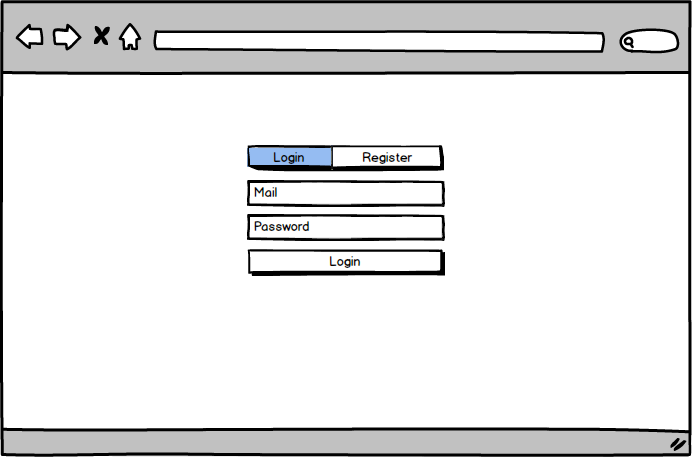
\includegraphics[width=0.7\linewidth]{kapitel1/mocks/Login.png}
 \caption{Login Screen Mock}
  \label{fig:login}
\end{figure}

\begin{figure}[h]
 \centering
 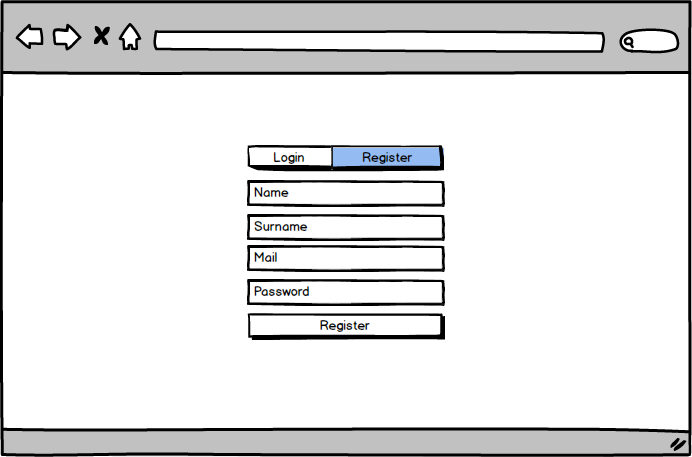
\includegraphics[width=0.7\linewidth]{kapitel1/mocks/Register.png}
 \caption{Register Screen Mock}
  \label{fig:register}
\end{figure}


\textbf{Login Formular}
\begin{itemize}
\item Mail (String, valide Mailadresse, eindeutig im System)
\item Password (String)
\end{itemize}

\textbf{Register Formular}
\begin{itemize}
\item Name (String)
\item Surname (String)
\item Mail (String, valide Mailadresse, eindeutig im System)
\item Password (String)
\end{itemize}



\subsubsection{System wählen / erstellen}

Da ein Nutzer in der Lage ist mehrere aktive Systeme zeitgleich zu monitoren,
wird eine Übersichtsseite (Abbildung \ref{fig:system-picker}) benötigt
um Systeme wechseln zu können. Zusätzlich sollen auf dieser Übersicht
neue Systeme angelegt werden können.

\begin{figure}[h]
 \centering
 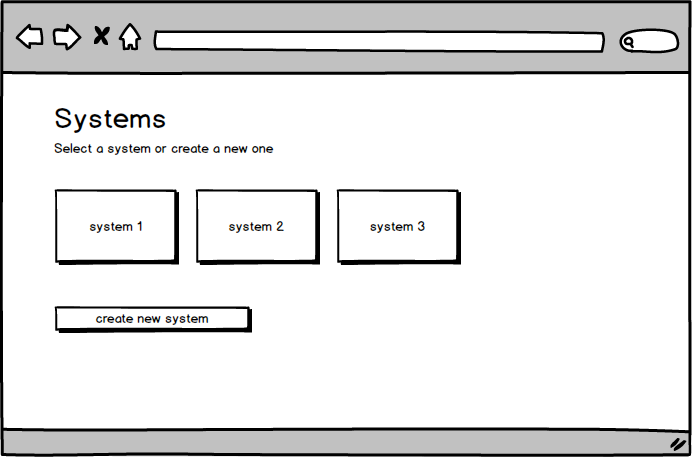
\includegraphics[width=0.6\linewidth]{kapitel1/mocks/system-picker.png}
 \caption{System wählen Mock}
 \label{fig:system-picker}
\end{figure}

\textbf{System erstellen}

\begin{itemize}
\item Name (String, maximal 20 Zeichen)
\item Beschreibung (String, maximal 255 Zeichen)
\end{itemize}


\subsubsection{Dashboard}

Auf dem Dashboard soll ein Nutzer die wichtigsten Informationen über sein System erhalten.
Fehlerverhalten des Systems soll deutlich und informativ dargestellt werden.
Zusätzlich soll das Dashboard als Einstiegspunkt für weitere Views dienen.

\subsubsection{Metriken}

Die Metriken-Sektion soll pro Applikation eine Kollektion von Diagrammen beinhalten.
Dabei soll die Applikation sowie der aktive Beobachtungszeitraum gewählt werden können.

\begin{figure}[h]
 \centering
 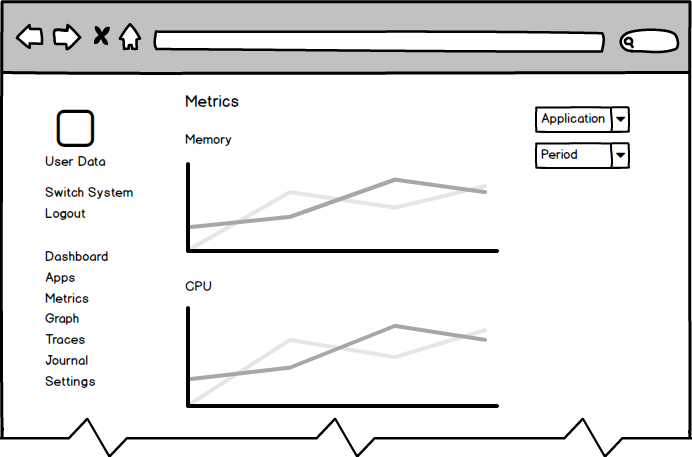
\includegraphics[width=0.6\linewidth]{kapitel1/mocks/metrics.png}
 \caption{Metrik Mock}
  \label{fig:metrics}
\end{figure}

\textbf{Diagramme}

\begin{itemize}
\item CPU Load
\item Memory
\item Requests client send
\item Requests server receive
\end{itemize}


\subsubsection{Graph}

Im Vergleich zur Metriken-View soll der Graph nicht nur einzelne Applikationen darstellen,
sondern das Kommunikationsnetz des Gesamtsystems visualisieren.
Wie in Abbildung \ref{fig:graph} zu sehen ist, sollen dabei Services als Knoten und Requests als Kanten dargestellt werden.
Bei den zu visualisierenden Metriken handelt es sich um die Faktoren Anzahl und Dauer der Requests zwischen den Services.
Zusätzlich soll auch hier der Beobachtungszeitraum definiert werden können.

\begin{figure}[h]
 \centering
 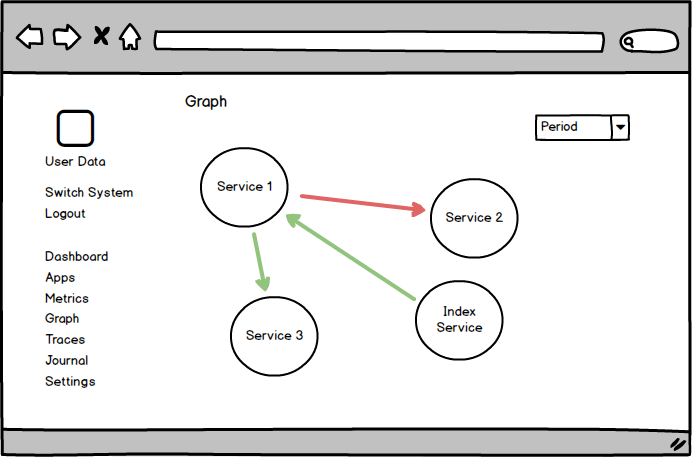
\includegraphics[width=0.6\linewidth]{kapitel1/mocks/graph.png}
 \caption{Graph Mock}
 \label{fig:graph}
\end{figure}

\subsubsection{Traces}

Die Traces Sektion besteht aus zwei verschiedenen Ansichten. Einer Übersichtsliste der Request Einstiegspunkte,
welche zur Trace Detailseite (Abbildung \ref{fig:trace}) überleitet. Im Detail besteht ein Trace aus den Requests
aller an einer Aktion beteiligten Services. Dabei werden die Service-Zugriffe in relation zur Zeit in einem Gantt Chart dargestellt.

\begin{figure}[h]
 \centering
 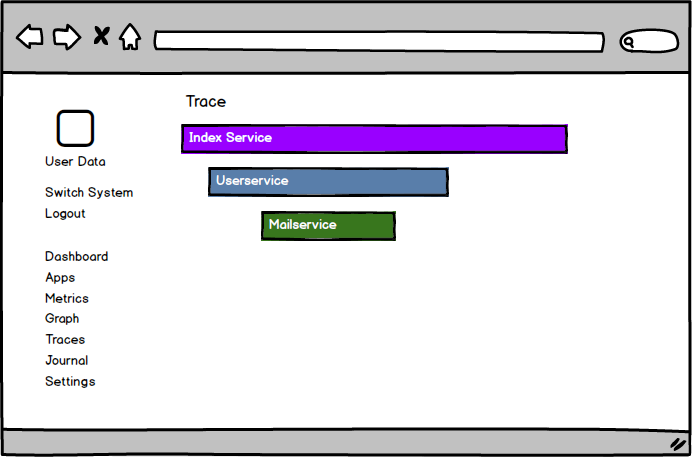
\includegraphics[width=0.6\linewidth]{kapitel1/mocks/trace.png}
 \caption{Trace Detailseite Mock}
 \label{fig:trace}
\end{figure}


\subsubsection{Journal}

\begin{figure}[h]
 \centering
 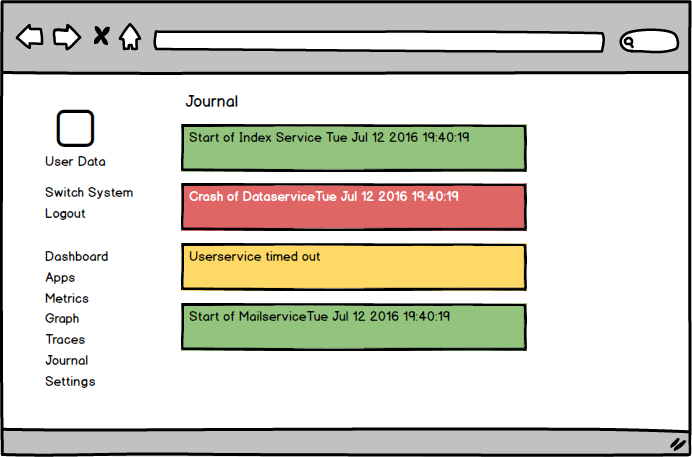
\includegraphics[width=0.6\linewidth]{kapitel1/mocks/journal.png}
 \caption{Journal Mock}
 \label{fig:journalmock}
\end{figure}

Das Journal (Abbildung \ref{fig:journalmock}) beinhaltet Einträge bezüglich Serverstart, Serverstop und Servercrash.


\subsubsection{Settings}

In den Einstellungen können Nutzerrelevante Parameter definiert werden. Metadaten können geändert werden
und Nutzer sollen die Möglichkeit erhalten ein Profilbild einzustellen.

\subsubsection{Events}

Reaktiv werden Nutzer auf Fehlverhalten ihrer Applikationen hingewiesen. Sollten Services außerplahnmäßig terminieren oder ihre Erreichbarkeit verlieren,
wird dies als Event, also als Notification, für den User ausgegeben.

\paragraph{mögliche Events}
\begin{itemize}
\item Service Start
\item Service Stop
\item Service Absturz
\item Anstieg von Request Latenzzeiten
\end{itemize}


\subsection{Plattformen}

Applikationen können anhand von Diagrammen und Graphen im Detail analysiert werden,
ferner möchte ein Nutzer reaktiv über Vorgänge seines Systems informiert werden, speziell wenn Latenzprobleme und Service-Ausfälle reibungslose Abläufe eines Systems gefährden.
Hierzu erhält der Nutzer Push Notifications über das Event System.

Die Applikation soll daher als App für iOS und Android sowie als Desktop Applikation für MacOS, Linux und Windows zur Verfügung stehen.
In Anbetracht, dass das Frontend Team nur aus meiner Person besteht, stellt sich diese Anforderung, in der doch knappen Entwicklungszeit, als große Herausforderung dar.
Daher liegt die Entscheidung nahe, den Ansatz der hybriden App Entwicklung zu wählen, statt die Applikationen für die jeweilige Plattform nativ zu implementieren.

%!TEX root = ../thesis.tex

\chapter{Grundlagen}

Im Folgenden werden Grundlagen erläutert die als Basis des Projekts sowie zum Verständnis von Kapitel \ref{chap:frameworks} Frameworks und Tools erforderlich sind.


\section{Native Entwicklung}

Bei der Entwicklung nativer Applikationen wird Prorammcode speziell für eine Zielplatform mit dem entsprechendem \ac{SDK} der Plattform entwickelt.
Die App ist damit an die Platform gebunden. Apps für Apples iOS werden in Swift oder Objective-C entwickelt und nutzen UIKit als Framework für die visuelle Darstellung.
Android Apps werden typischerweise in Java implementiert und nutzen das Android Framework als Systemschnittstelle und für die Entwicklung des \ac{UI}.
Nativ entwickelte Apps werden als Binärdatei über den jeweiligen Appstore verteilt und auf das Gerät installiert \cite{Heitkoetter2013}.

\vspace{0.3cm}
\textbf{Desktop Nativ}
\begin{itemize}
\item macOS (Swift, ObjectiveC, Java)
\item Linux (C++, C\#, Java)
\item Windows (C++, C\#, VisualBasic, Java)
\end{itemize}
\vspace{0.3cm}

\textbf{Mobil Nativ}
\begin{itemize}
\item iOS (Swift, ObjectiveC)
\item Android (Java)
\end{itemize}
\vspace{0.3cm}

\section{Mobile Cross Platform Entwicklung}

Im Vergleich zum Ansatz der nativen Entwicklung bieten diverse Cross-platform Entwicklungsansätze die Möglichkeit, eine Codebasis zu entwickeln,
die auf diversen Platformen ausgeführt werden kann \cite{Heitkoetter2013}.
Hierbei muss zwischen Browserbasierten Web Apps (Cordova, Phonegap) und Cross kompilierten Applikationen (Xamarin, Titanium, FireMonkey) unterschieden werden
\cite{Xamar84:online}.

\subsection{Cross-kompilierte Apps am beispiel von Xamarin}

Xamarin Entwickler können den in C\# geschriebenen Code für die Plattformen iOS, Windows Mobile und Android kompilieren.
Der resultierende Code läuft dabei als nativer Code auf den Geräten.
Die Xamarin Entwickler versprechen, dass alles was in Swift, Objective-C und
Java möglich ist, auch mit C\# und Xamarin umgesetzt werden kann \cite{projectxamarin}.

\begin{figure}[ht]
 \centering
 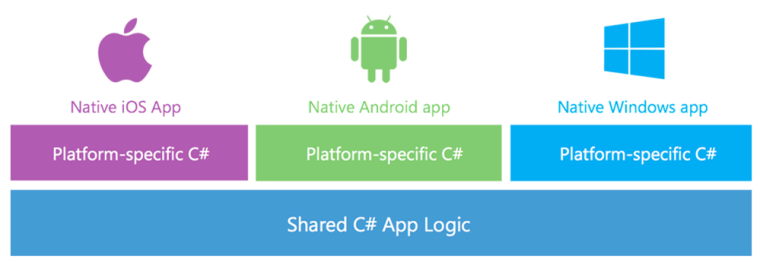
\includegraphics[width=0.9\linewidth]{kapitel2/csharp_xamarin.png}
 \caption{Xamarin Platforms \cite{7Reas20:online}}
\end{figure}
\vspace{1cm}

Xamarin stößt bezüglich \ac{UI} schnell an seine Grenzen. Das \ac{UI} Layer muss aufgrund von Kompatibilitätsproblemen und fehlender Features des Xamarin Framework
für jede Platform indiviudell entwickelt werden. Das funktioniert, wenn die App entsprechend dem Plattform CI umgesetzt werden soll und sich die \ac{UI} so weit unterscheidet,
dass Abstraktionen und komponentenbasierte Entwicklung vernachlässibar sind, jedoch ist es fragwürdig ob sich das Framework als ``Cross Plattform Frontend Framework'' bezeichnen darf,
wenn ein Großteil der Implementierung, zumindest bei Plattform-universellem Appdesign, nach wie vor redundant vorgenommen werden muss \cite{7Reas20:online}.

\begin{figure}[ht]
 \centering
 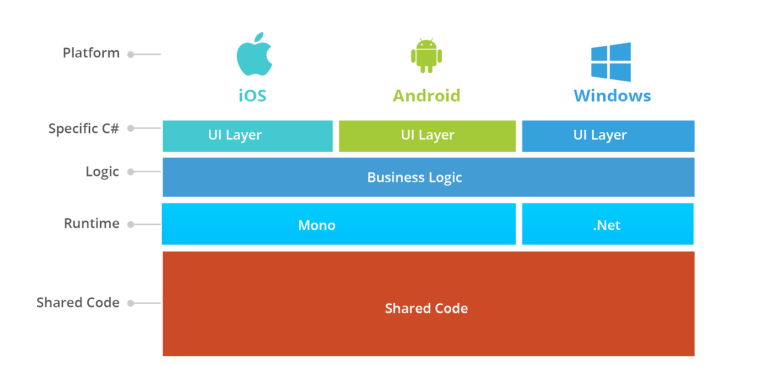
\includegraphics[width=0.8\linewidth]{kapitel2/xamarin_ui_blocker.png}
 \caption{Xamarin Layer \cite{7Reas20:online}}
\end{figure}

\newpage


\subsection{Web Apps (Cordova, Phonegap)}

Cordova ist ein Framework von Adobe Systems um Mobile Cross Plattform Anwendungen mithilfe von Webtechnologien zu entwickeln.
\ac{HTML}, \ac{CSS} und JavaScript werden genutzt um Produkte für iOS, Android, Ubuntu, Blackberry OS, Firefox OS und Windows Phone zu generieren \cite{Cordo26:online}.
Der Code wird, im Vergleich zu mit Xamarin entwickelten Apps, nicht für verschiedene Plattformen kompiliert,
sondern läuft in einer nativen Webview. Diese Apps werden auch als hybride Apps bezeichnet.
Ionic und Phonegap sind Frameworks, die auf der Cordova Technologie aufsetzen.

Zugriff auf Systemschnittstellen erhält man mittels Cordova Plugins. Diese bieten
Interfaces in Javascript für den Zugriff auf native Systemkomponenten wie Kamera, GPS, Dateisystem etc.
Plugins bestehen daher aus Javascript und dem Plattform kompatiblen Code,
also beispielsweise Swift/Objective-C für iOS oder Java für Android.

\ac{UI} Entwicklung muss im Vergleich zum Xamarin Framework nicht redundant vorgenommen werden, da Implementierungen der
Ansichten für sämtliche unterstützten Plattformen identisch ausgeliefert werden können.
Da \ac{UI} mithilfe von \ac{HTML} und \ac{CSS} realisiert wird,
können spezielle Stilregeln dennoch auch plattformspezifisch angewandt werden, um beispielsweise eine App zu entwickeln,
welche den jeweiligen Stil Richtlinien der Plattformen entsprechen soll.

\vspace{1cm}
\lstinputlisting[language=Java,label=code,caption=Cordova Kamera Example]{kapitel2/cordova-plugin-example.js}
\vspace{1cm}

\newpage
\section{Web Components}


\subsection{Einführung}

Moderne Webanwendungen bestechen heutzutage meist nicht nur mit ihrem komplexen Design, Komplexität lässt sich auch in der Entwicklung
von Funktionalität nicht vermeiden. Dieses Problem wird noch brisanter, wenn eine Applikation über einen langen Zeitraum hinweg,
womöglich von verschiedenen Entwicklerteams, entwickelt und betreut wird. Mit Blick auf das \ac{DOM} von Patrioten moderner und komplexer Webanwendungen wie Facebook, Ebay oder Amazon
wird schnell klar, dass deren Domstruktur durch Inflationäre Nutzung von DIV und SPAN Tags schnell zu Unübersicht führt,
da die Palette an HTML5 Semantic Tags nicht ausreicht um die Funktionalitäts Vielfalt einer modernen Webanwendung zu beschreiben.
Statt aussagekräftige Tags zu verwenden, müssen Klassen und IDs zweckentfremdet werden, um HTML Elemente überhaupt voneinander unterscheiden zu können
\cite{sitepoint-introduction-to-webcomponents}.

\subsection{Komponenten in der Softwarentwicklung}

``Modern applications are increasingly
open in terms of topology,
platform and evolution, and so the
need for a component-oriented
approach to development is even
more acute than in the past [...]  Objects provide an organizational
paradigm for decomposing large
applications into cooperating objects
as well as a reuse paradigm for
composing applications from prepackaged
software components.''
\cite{nierstrasz1992component}

\vspace{0.5cm}

Bereits 1992 sprachen Nierstrasz, Gibbs und Tsichritzis vom Traum der komponentenorientierten Softwareentwicklung.
Dabei soll Software aus vielen Komponenten aufgebaut werden, im Idealfall habe man die Möglichkeit ein
ganzes Set an vorgefertigten Komponenten für die Konstruktion seiner Applikation zu verwenden.
Hierbei soll der Aspekt der Abstraktion und Wiederverwendbarkeit durch Objektorientierung von zentraler Bedeutung sein.

\vspace{0.5cm}
``A software component is a unit of composition with contractually specified interfaces and explicit
context dependencies only. A software component can be deployed independently and is subject to composition
by third parties.''
\cite{Szyperski}
\vspace{0.5cm}

Szyperski definiert eine Komponente als eigenständiges, in sich geschlossenes Modul ohne Deployment
Abhängigkeiten, d.h. Eine Komponente kann ausgeliefert werden, ohne dass andere Elemente der Applikation ebenfalls neu gebaut werden müssen.
Klar definierte Schnittstellen dienen der komponentenübergeifenden Kommunikation und repräsentieren
dabei die Funktionalität der Komponente möglichst Transparent.
Komponenten sollen dabei angeboten, sei es komerziell oder gratis,
und von Dritten verwendet werden können.


\subsection{Web Components}

``Web Components are an emerging set of standards from the W3C to describe a way to create encapsulated,
reusable blocks of UI presentation and behavior entirely with client side languages- HTML, JavaScript and CSS.''
\cite[42]{Web-Component-Architecture}
\vspace{1cm}

Der W3C beschreibt diverse Wege, wie entkoppelte wiederverwendbare UI Elemente, sogenannte Web Components,
in Kombination von \ac{HTML}, JavaScript und \ac{CSS} geschaffen werden können.
Der Begriff Web Components beinhaltet eine Sammlung von Standards,
welche die bereits genannte Problematik der fehlenden HTML Semantik mit bestehenden Webtechnologien lösen kann.
Web Components funktionieren als wiederverwendbare Web Widgets mit klar definierten Schnittstellen.
Dabei sollen sie im Browser implementiert und ohne externe Bibliotheken nutzbar sein.
Bestehende Web Komponenten sollen ohne zusätzlichen Code funktionsfähig sein. Lediglich durch das Einfügen der Komponente
in das Markup, soll bereits die komponenteninterne Funktionalität zur Verfügung stehen
\cite[42]{Web-Component-Architecture}.
Webcomponents bauen auf vier Kerntechnologien auf: HTML Imports, HTML Teamplates, Custom Elements und Shadow Dom.

\subsubsection{HTML Imports}
HTML kann in HTML Dokumente importiert und verwendet werden.
Dabei können in dem referenziertem zu importierendem HTML Abhängigkeiten in Form von CSS und JS eingebunden werden,
welche dementsprechend aufgelöst werden.
Sollten mehrere Dokumente mit der selben Abhängigkeit eingebunden werden, wird diese dennoch nur einmalig geladen
\cite{HTMLI44:online}.

\vspace{0.3cm}
\lstinputlisting[language=HTML,label=code,caption=HTML Imports]{kapitel2/html_import.html}
\vspace{0.3cm}

\subsubsection{HTML Templates}

Das HTML Template-Element ermöglicht Inhalte nicht zur Laufzeit der Website zu rendern,
sondern den Rendervorgang explizit per JavaScript zu steuern. Ressourcen wie Videos und Bilder werden demnach
nicht initial geladen und erzeugen keine unnötige Ladeverzögerung der Applikation.
Inhalte des Template-Tags werden zu Beginn auf Validität geprüft und stehen dann für die Verwendung im Dokument
zur Verfügung.

\subsubsection{Custom HTML Elements}

Durch Custom HTML Elements werden Webkomponenten in Applikationen eingebunden.
Eigene HTML Tags und Elemente können definiert werden und beinhalten in Javascript geschriebene Logik sowie CSS Styling.
Ein Custom Element besitzt einen Lifecycle mit diversen Einstiegspunkten:

\begin{itemize}
\item createdCallback - Element wird registriert
\item attachedCallback - Element wird in den DOM der Applikation eingefügt
\item detachedCallback - Element wird aus dem DOM entfernt
\item attributeChangedCallback - Attribute werden Elementen hinzugefügt, verändert oder entfernt
\end{itemize}


\subsubsection{Shadow Dom}
Shadow Dom ermöglicht Optik und Logik einer Komponente zu kapseln.
Seiteneffekte, bezüglich komponentenübergreifendem Style und Logik, werden verhindert.
Beispielsweise kann das Styling eines Menüs nicht aufgrund gleicher CSS Prefixe den Style des Contents überschreiben,
da dieser in die Navigations-Komponente gekapselt ist und nicht auf die globalen Styles des Dokuments oder anderer Elemente zugreifen kann.
Webapplikationen lassen sich dadurch paketweise organisieren und strukturieren.

\subsubsection{Polyfills}

\vspace{1cm}
\begin{figure}[htp]
 \centering
 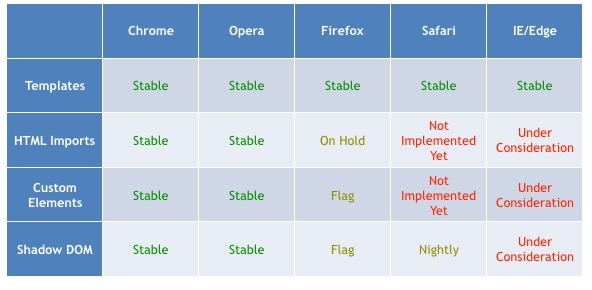
\includegraphics[width=0.8\linewidth]{kapitel2/platform_support.jpg}
 \caption{Platform Support}\cite{WebCo43:online}
 \label{fig:platform_support}
\end{figure}

Wie in Abbildung \ref{fig:platform_support} zu sehen ist, sind Web Components noch nicht in
allen gängigen Browsern nativ verfügbar. Lediglich in Chrome und Opera sind diese implementiert.
Hier kommen Polyfills ins spiel. Polyfills implementieren fehlende Browserfeatures und gewährleisten damit beispielsweise nahezu Vollständigen
Support von Web Components in allen gängigen Browsern. Ein weiteres Beispiel für ein Polyfill ist core-js,
welches die die Nutzung der JavaScript Standards ES5 und ES6, auch wenn der Browser diese nicht unterstützt, ermöglicht.



\section{Typescript}

\subsection{Entwicklung von Javascript}

\begin{figure}[ht]
 \centering
 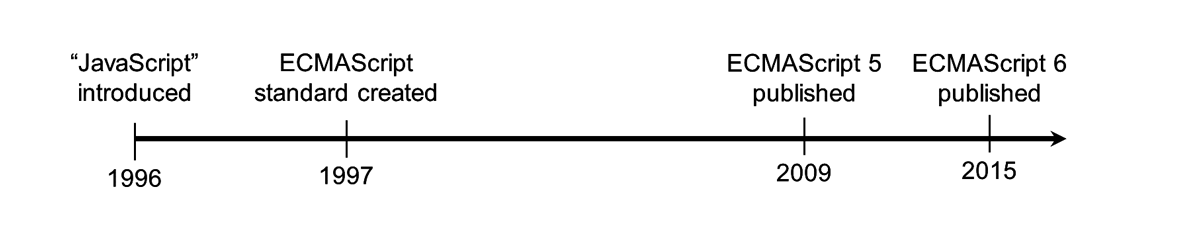
\includegraphics[width=\linewidth]{kapitel2/javascript-timeline.png}
 \caption{History of Javascript}\cite[28]{EssentialTS}
\end{figure}

Javascript wurde erstmals 1996 von Brendan Eich in einer Implementierung des Netscape Navigator Browsers eingeführt,
worauf weitere Browser die Syntax und APIs ähnlich, jedoch nicht identisch nach implementierten.
Daraufhin veröffentlichte die ECMA International einen Standard, welcher die Spezifikationen der neuen Sprache
definieren sollte. Dieser trägt den namen ECMAScript und ist der offizielle und bekannteste Standard der
Sprache. ActionScript von Macromedia und JScript von Microsoft sind weitere Implementierungen der Browsersprache,
die nicht dem ECMA Standard entsprechen, jedoch darauf aufbauen.

1997 wurde die erste Version des nun standardisiertem ECMAScript veröffentlicht. Ein Jahr später erschien bereits ECMAScript2,
allerdings beinhaltete dieses Update nur kleine Änderungen um einem parallel entstandenen ISO Standard von JavaScript zu implementieren.
Die nächste große Neuerung kam 1999 mit ECMAScript3, in welcher einige innovative Features implementiert wurden.
``[...]regular expressions, better string handling, new control statements, try/catch exception handling, tighter definition of errors, formatting for numeric output and other enhancements.''\cite{js-vs-es}.

Das nächste Update ECMAScript4 war 2008 geplant, zunächst als Prototyp entwickelt,
jedoch noch vor dem Release aufgrund eines rückschritttigem Featureset wieder aufgegeben.
Zur selben Zeit etstand Ajax und damit eine völlig neue Art von dynamsichen Webapplikationen,
basierend auf JavaScript.

2009 erschien ECMAScript5 und erhielt kurz darauf vollen Support in nahezu allen verbreiteten Webbrowsern, abgesehen vom Internet Explorer.
Es beinhaltet neue Features wie \ac{JSON} Support und klassische Array Funktionen wie map und forEach.
Durch die Entfernung einiger Features wurde JavaScript in der neuen Version sauberer und stabiler.

ECMAScript6 sollte bereits 2013 veröffentlicht werden, der offizielle Releasetermin wurde
dann allerdings bis in den Juni 2015 verschoben und ist bis heute noch nicht ausreichend in allen Browsern implementiert
\cite{js-vs-es}.

\subsection{Allgemein}

Typescript ist eine von Microsoft entwickelte Programmiersprache.
Die Sprache ist ein Superset von ES6, d.h. sie implementiert den JavaScript Standard und ergänzt diesen
durch zusätzliche Features, wie der statischen Typisierung.
Typescript will ausgereifter, robuster und speziell in großen Projekten eine solidere Alternative sein \cite[28]{EssentialTS}.
Zusammen mit ES6 erhalten Entwickler gegenüber ES5 folgende Features:

\begin{figure}[ht]
 \centering
 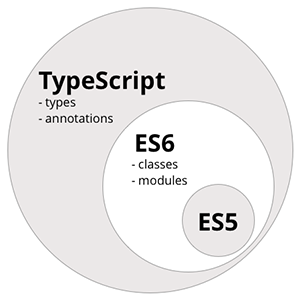
\includegraphics[width=0.4\linewidth]{kapitel2/typescript----es5-es6-typescript-circle-diagram.png}
 \caption{Language Relationship}\cite[152]{ng-Book-2}
\end{figure}


\subsubsection{statische Typisierung}

Die wohl größte Errungenschaft der Sprache ist das statische Typsystem.
Typenfehler können in Typescript bereits zum Zeitpunkt
der Kompilierung bzw. Transpilierung erkannt werden und treten nicht erst zur Laufzeit im Browser auf.
Zudem wird Code in einer Typescript unterstützenden IDE dank Autovervollständigung
leichter zu schreiben und aussagekräftiger zu lesen \cite[156]{ng-Book-2}.

\subsubsection{Klassen}

Mit ES6 Klassen wurde eine neue Syntax für das prototypische Vererbungsmodell von Javascript entwickelt.
Dabei handelt es sich nicht um die Einführung eines neuen OOP-Modells, sondern lediglich um eine vereinfachte Syntax für Objekte und deren Schnitstellen,
sowie die Realisierung von Abstraktionen, wie sie aus anderen Objektorientierten sprachen wie C++, Swift oder Java bereits bekannt sind.\cite{js-Klassen}

\lstinputlisting[language=Java,label=code,caption=Klassen in ES6]{kapitel2/class.js}

\subsubsection{Module}

In ES5 gab es keinen Standard um Funktionen und Variablen in Namensräumen zu organisieren oder dynamisch Code zu laden.
Mit ES6 wurde das fehlende Feature durch das Exportieren und Importieren von Modulen ergänzt. Dadurch wird es sehr bequem, Programmcode zu organisieren und zu laden.
Jedes ES6 Modul wird in einer eigenen Datei gespeichert. Variablen und Funktionen sind von außerhalb nicht sichtbar, es sei denn, sie werden explizit exportiert.
Mittels Export lassen sich also Schnittstellen für ein Modul definieren, welche importiert und verwendet werden können.
In Typescript lassen sich ganze Klassendefinitionen exportieren.
Dabei ist es möglich, Instanzfunktionen und Instanzvariablen mit dem Keyword private vor dem äußeren Zugriff zu verstecken.
Public Funktionen sind dann auch von außen nutzbar.

\lstinputlisting[language=Java,label=code,caption=Export und Import von Modulen in ES6]{kapitel2/module.js}

\subsection{Transpilierung}

Typescript sowie ES6 bieten Entwicklern eine ganze Reihe von Neuerungen gegenüber den Vorgängerversionen.
Spannende Features bringen jedoch wenig, wenn sie im Standard zwar spezifiziert wurden,
allerdings noch in sehr wenigen Browsern vollständig implementiert sind.
Um TS oder ES6 Code also überhaupt in Produktion zu nutzen, sollte er auf den ES5 oder ES3
Standard herunter transpiliert werden.
Ein Transpiler ist ein Compiler, welcher Sourcecode nicht in Maschinencode, sondern ebenfalls in Sourcecode,
allerdings einer anderen Sprache oder Sprachversion wandelt \cite{Introduction-to-the-Typescript-Transpiler}.
In der nachfolgenden Abbildung ist zu sehen, wie Typescript-Code in funktionsfähigen ES5 Code transpiliert wird.

\begin{figure}[ht]
 \centering
 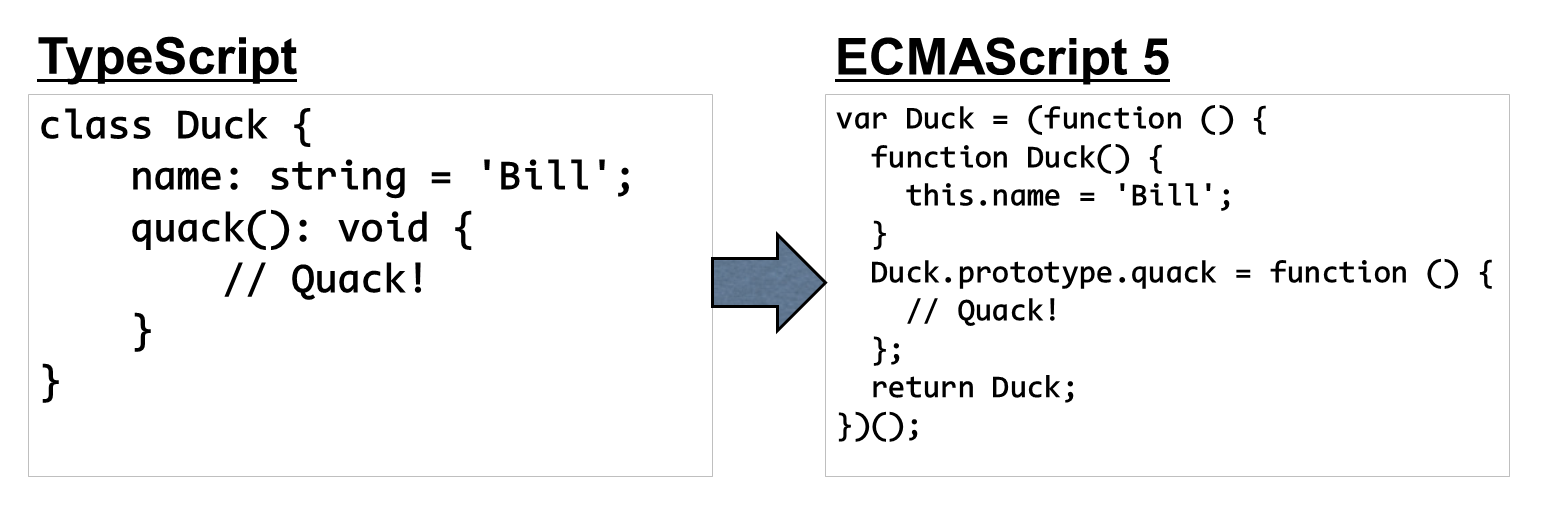
\includegraphics[width=0.8\linewidth]{kapitel2/Introduction-transpiler.png}
 \caption{Transpilierung}\cite[27]{ng-Book-2}
\end{figure}

%!TEX root = ../thesis.tex

\chapter{Frameworks und Tools}
\label{chap:frameworks}

Im Folgenden werden die für den praktischen Teil der Arbeit genutzten Frameworks und Tools beschrieben.
Ziel dieses Kapitels ist es, die Auswahl der genannten Frameworks zu begründen und
ihren Funktionsumfang hinsichtlich der Projektanforderungen zu untersuchen.

\section{AngularJS}

Angular ist derzeit eines der populärste Frontend Javascript Frameworks auf dem Markt.
Böhm war einer der ersten Entwickler, der Angular 2012 in Deutschland bekannt machte.
``Zu dieser Zeit war jQuery noch die Basis des Webs. jQuery hatte aber nie den Anspruch, ein Framework für Web-Anwendungen zu sein. Der eigentliche Sinn war, die APIs der verschiedenen Browser zu vereinheitlichen.
Man musste sich deshalb immer eine eigene Architektur überlegen. Allerdings fehlte die Erfahrung, wie man große Applikationen im Web schreibt. Das führte natürlich oft zu Chaos und unwartbaren Projekten.''\cite{Angu68:online}
Böhm spricht mit Angular von einem sehr mächtigen Komplettpaket, welches Anwendungsentwicklung im Web auf ein neues Level hebe.
Gründe dafür sind die geringe Lernkurve, simple Template Syntax,
welche auf \ac{HTML} aufbaut sowie hohe Wartbarkeit aufgrund einfacher Testbarkeit von einzelnen Anwendungskomponenten.

Böhm bezeichnet Angular 2 als ein Framework für die Zukunft.
Anwendungen, die zeitnah in Produktion gehen sollten, würde er nach wie vor mit Angular 1 entwickeln,
da Angular 2 noch nicht als Release vorliegt und interne Funktionalität auf Browserfeatures basiert,
die teilweise noch nicht in jedem Browser zur Verfügung stehen und daher durch Polyfills implementiert werden müssen.
``Somit wird Angular 2 sein ganzes Potential wohl auch erst in einigen Jahren entfalten können.
Wenn man jedoch erst heute damit anfangen würde, ein Framework für heute zu bauen,
ist es bereits veraltet, wenn es fertig ist.''\cite{Angu68:online}
Zudem sind Styleguides und Best Practise Ansätze für die Entwicklung von Applikationen mit Angular 2
noch in der Entstehung.
Dennoch ist Böhm von den Konzepten von Angular 2 überzeugt.


\subsection{Neuerungen des Frameworks}

Angular 2 ist die Nachfolgeversion des von Google entwickelten JavaScript Framework Angular 1.
Die 2009 veröffentlichte erste Version fand großen Anklang in der Community
und wurde als Basis für dynamische Single-page-Webanwendung verschiedenster Art und Größe genutzt.
In den seit dem Release vergangenen Jahren hat sich die Community um das Framework immer weiter vergrößert,
welche zur stetigen Weiterentwicklung und so zu dem Erfolg von Angular 1 beigetragen hat.
Das Github Repository der ersten Version hat mittlerweile 1.489 Contributors mit nahezu 7000 gestellten Pull Requests \cite{ng1-github}.

Mit Angular 2 wurden einige Grundkonzepte überarbeitet, um in eine komplett neue Richtung gehen zu können.
Ziel von Google ist es, ein komponentenbasiertes und leicht bedienbares Framework für moderne
Webanwendungen zu schaffen, das Performanceverbesserungen und transparentere interne Strukturen als die Vorgängerversion aufweisen soll.
Eine Angular 2 Anwendung besteht daher aus einer Vielzahl diverser Komponenten, wodurch es möglich wird,
Funktionalität zu kapseln, zu abstrahieren und wieder zu verwenden. Der Fokus hierbei liegt nicht nur auf Wiederverwendbarkeit innerhalb einer Codebasis.
Elemente der Anwendung sollen sowohl für den Browser als auch für mobile Geräte sowie für native Desktop Clients genutzt werden können.
Angular 2 soll im Vergleich zu seiner Vorgängerversion leichter zu lernen und zu nutzen sein,
sowie auch für komplexere Webanwendungen eine solide Basis bieten \cite[11-12]{Angular2}.


\subsection{Komponenten}

Komponenten sind die Grundbausteine einer jeden Angular 2 Applikation und ersetzen Direktiven aus Angular 1 nahezu vollständig.
UI und deren Funktionalität wird innerhalb von Komponenten implementiert.
Diese werden in Angular 2 als Typescript Klasse definiert und mit @Component dekoriert, siehe Listing \ref{ng2component}.
Der Component Decorator wird mithilfe des ES6 Imports importiert (Zeile 1) und wird verwendet um die Klasse mit erforderlichen Metadaten zu auszustatten.
Der Selektor (Zeile 5) definiert den HTML Tag der Komponente, über welchen diese innerhalb der Anwendung eingefügt und damit instanziiert werden kann.

Template beziehungsweise TemplateUrl in Zeile 7 enthält entweder einen String mit inline Markup in angulars Template Syntax
oder eine Referenz zu einer zugehörigen HTML Datei, welche das Markup der Komponente enthält.
Ebenso kann \ac{CSS} inline oder per Dateireferenz (Zeile 8) eingebunden werden.
Über Directives (Zeile 6) können Komponenten referenziert werden, welche innerhalb dieser Komponente verwendet werden sollen.
Ist eine Komponente als Directive referenziert,
kann ihr Selector im Markup eingebunden,
und dadurch ihre gesamte Funktionalität genutzt werden.

Die Komponentenklasse hat einen Klassennamen und einen impliziten oder expliziten Konstruktor.
Sie wird mithilfe des ES6 Prefixes öffentlich exportiert (Zeile 11).
Die Sichtbarkeit von Variablen und Funktionen innerhalb der Klasse kann mithilfe der Prefixe private und public definiert werden.
Dadurch ist es möglich, Funktionalität und Daten innerhalb einer Komponente, transparent für deren Verwender, zu kapseln.
Die Implementierung der Angular Komponenten basiert dabei auf dem Standard der Web Components, welcher bereits in \ref{sec:webcomponents} Web Components beschrieben wurde.

\newpage

\lstinputlisting[language=Javascript,label=ng2component,caption=Basic Component]{kapitel3/basic-component.ts}


\subsubsection{Vererbung}

Vererbung ist eines der Grundkonzepte von Objektorientientierung,
welches eingesetzt wird, um Verhalten von Objekten bezüglich Wiederverwendbarkeit zu
abstrahieren. Angular 2 Komponenten bestehen aus Klassen, daher
kann Vererbung genutzt werden um Funktionalität von Komponenten zu abstrahieren,
um redundanten Code zwischen den Komponenten
zu vermeiden. Funktionalität wird dabei von der Komponente in eine dritte Klasse ausgelagert,
welche mit dem Schlüsselwort extend als
Abstraktionsebene eingebunden wird \cite{DanWa45:online}.

\subsubsection{Lebenszyklus}
Eine Angular Komponente besitzt einen Lebenszyklus (Component Lifecycle) mit diversen Einstiegspunkten,
um wichtige Momente einer Angular Komponente für die Entwicklung offen zu legen \cite[837-839]{ng-Book-2}.
Zur Verdeutlichung sind einige dieser in Listing \ref{lifecycle-example} implementiert.
NgOnInit und ngOnDestroy werden beispielsweise zum Zeitpunkt der Instanziierung und Dekonstruktion der Komponente aufgerufen.
Angular führt ngOnChanges aus, wenn sich Variablen der Komponente verändert haben. Anhand von SimpleChanges
können Daten vor und nach dem Event miteinander verglichen werden.
Wie Angular die Änderung von Variablen ermittelt, wird in \ref{sec:change-detection} Change Detection erläutert.

\newpage


\lstinputlisting[language=Java,label=lifecycle-example,caption=Lebenszyklus Beispiel]{kapitel3/lifecycle-example.ts}
\vspace{0.3cm}




\subsection{Services, Providers und Dependency Injection}
\label{sec:services}

Oftmals bietet es sich an, Funktionalität von Komponenten in Services auszulagern.
Speziell wenn mehrere Komponenten auf die selben Daten,
die womöglich asynchron per HTTP geladen werden müssen, zugreifen.
Services werden ebenfalls als Klassen implementiert, welche mithilfe von \ac{DI}
als Singleton instanziiert und in die Komponenten injiziert werden können.
\ac{DI} ist ein Design Pattern, welches bereits in der ersten Version des Frameworks implementiert war.
In Angular 2 wurde \ac{DI} neu entwickelt, um flexiblere Injizierung von Services in Komponenten zu ermöglichen.

\ac{DI} bringt vielerlei Vorteile mit sich. In der Implementierung einer Angular 2 Komponente wird im
Konstruktor deklariert, welche Abhängigkeiten (Dependencies) für die Komponentenfunktionalität benötigt werden.
Das Framework ist dabei für die automatische Instanziierung der Objekte verantwortlich.
Die Implementierung von Komponenten wird durch die Verwendung von \ac{DI} sehr dynamisch,
da Implementierungen von Services, wie in Abbildung \ref{service-injection} dargestellt, einfach ausgetauscht werden können.
Soll beispielweise die Funktionalität einer Komponente, welche über einen Service dynamisch Daten lädt, getestet werden,
so kann die Implementierung des Services einfach ausgetauscht werden, so dass dieser statische Testdaten liefert,
sollte der API-Server in der Testumgebung nicht erreichbar sein \cite[281]{Angular2}.


\vspace{0.3cm}

\begin{figure}[ht]
 \centering
 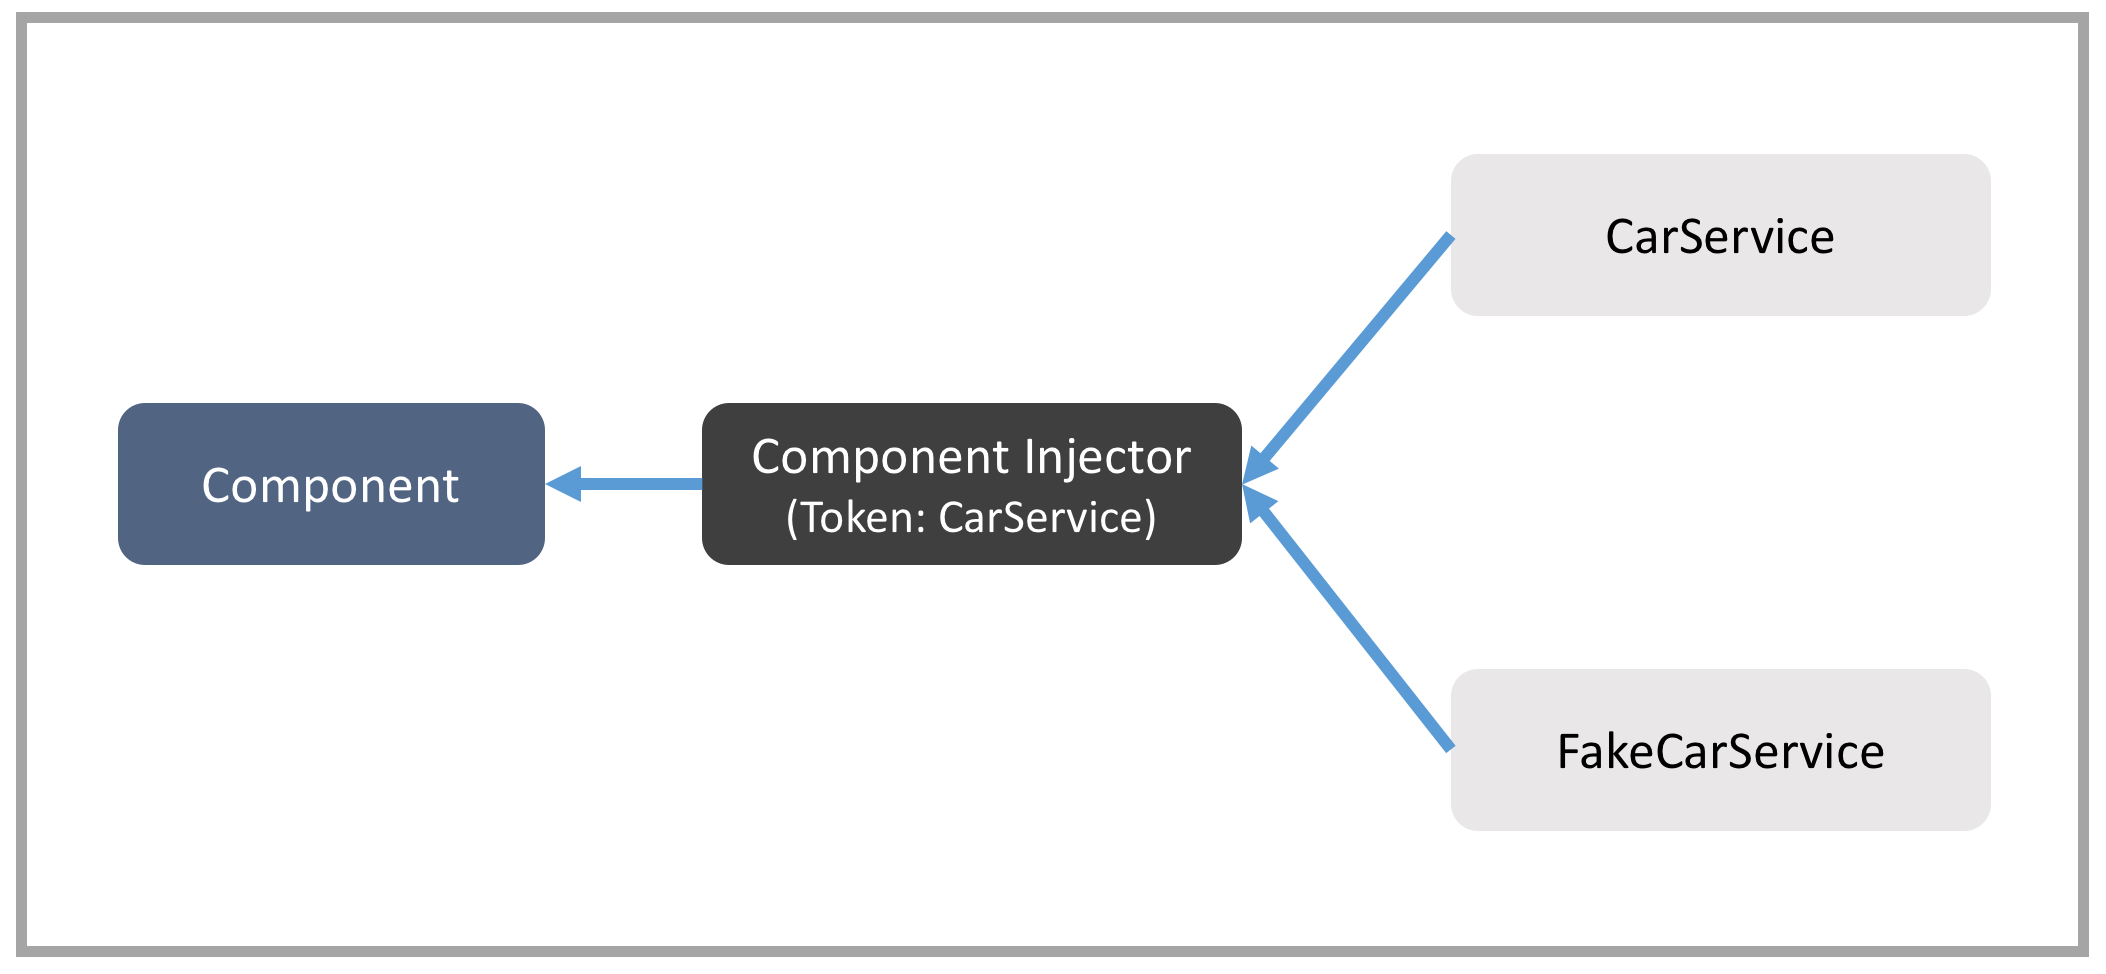
\includegraphics[width=0.8\linewidth]{kapitel3/component-injector.png}
 \caption{Component Injector}\cite[343]{Angular2}
 \label{service-injection}
\end{figure}
\vspace{0.3cm}

\ac{DI} wird in Angular mithilfe von Providern konfiguriert.
Dies geschieht auf Komponentenebene oder im Root der Applikation.
Wird ein Service über einen Provider im Bootstrap Prozess im Root der Applikation referenziert,
so ist diese Instanz des Services in jede Komponente der Applikation injizierbar.
Wird der Provider erst in der Komponente definiert (Listing \ref{provider2}), so ist die Serviceinstanz nur in dieser Komponente sowie in
allen Kindkomponenten verfügbar. Desweiteren lassen sich Provider kombinieren, da diese überschreibbar sind.
Sollte also ein Serviceprovider im Root der Applikation definiert sein (Listing \ref{provider1}), können dennoch weitere Provider in den Komponenten definiert werden.
Jedoch werden demnach auch mehrere Instanzen des Services erzeugt.
Es wäre also möglich, individuelle Singletons für bestimmte Komponentenbäume zu erzeugen \cite[286]{Angular2}.

\vspace{0.2cm}
\lstinputlisting[language=Javascript,label=provider1,caption=Provider im Bootstrap Prozess]{kapitel3/provider-example-root.ts}
\vspace{0.2cm}

\vspace{0.2cm}
\lstinputlisting[language=Javascript,label=provider2,caption=Provider in einer Komponente]{kapitel3/provider-example.ts}
\vspace{0.2cm}


\subsubsection{Services als Singletons}
\label{Services-als-Singletons}

Wie bereits erwähnt, ermöglichen \ac{DI} Provider Services als Singleton zu instanziieren.
Dies bringt viele architektonische Vorteile mit sich. Services können auf der einen Seite genutzt werden,
um Funktionalität aus Komponenten zu abstrahieren um in weiteren Komponeten verwendet zu werden.
Auf der anderen Seite können sie jedoch auch genutzt werden, um Daten multiplen Komponenten zur Verfügung zu stellen.
Das Angular Framework sorgt dafür, dass ein Service nur einmalig instanziiert wird. Daher erhalten alle
Komponenten, die den Service injizieren, die selbe Referenz, somit die selbe Instanz und daher die selbe globale Datenbasis.
In einem Userservice könnte beispielweise eine Boolean Variable definiert sein, welche Auskunft darüber gibt,
ob ein User eingeloggt ist oder nicht \cite[308]{Angular2}.


\subsection{Data Binding}
Das in eine Komponente eingebundene Markup repräsentiert die Viewschicht einer Komponente.
Angular 2 besitzt zur Darstellung von Datenstrukturen eine komplexe, jedoch sehr ausdrucksstarke Template Syntax, siehe Listing \ref{ngtemplate}.
Variablen und Funktionen einer Komponente, können mithilfe von doppelt geschweiften Klammern in die View eingebunden werden.
Auf der Basis von HTML5 können zudem Schleifen und Fallunterscheidungen implementiert werden.
Der Gültigkeitsbereich des Templates bezieht sich, bezüglich Variablen und Funktionen, dabei auf den Kontext der Komponente,
welche das Template in der Component Decoration referenziert \cite{Templ78:online}.

\vspace{0.3cm}
\lstinputlisting[language=HTML,label=ngtemplate,caption=Angular 2 Template Syntax]{kapitel3/template-example.html}

\subsection{Kommunikation}

Da eine Angular 2 Applikation ausschließlich aus Komponenten besteht, müssen diese zwangsweise miteinander
kommunizieren können. Für den Austausch von Daten gibt es verschiedene Ansätze.
Wie bereits in \ref{Services-als-Singletons} Services als Singletons erwähnt, werden Services im Normalfall als Singleton
instanziiert und in Komponenten mittels \ac{DI} injiziert. Öffentliche Servicefunktionen können hier für den
Austausch von Daten genutzt werden. Über den synchronen Zugriff auf Variablen hinaus,
können Events in Komponenten oder Services definiert und ebenfalls aboniert werden,
um asynchrone Kommunikation applikationsintern zu ermöglichen. Die Auslagerung von Funktionalität in Services ergibt jedoch nur dann wirklich Sinn,
wenn diese auch als Singleton existieren kann.

Komponenten sind im Vergleich zu Services keine Singletons,
da sie mit jeder Verwendung in der Applikation neu instanziiert werden.
Variablen und Funktionen eingebundener Komponenten können durch die Annotationen @Input und @Output
direkt über ihren HTML Component Tag angesprochen werden. Im Normalfall werden bei der Instanziierung von Kindkomponenten
relevante Daten über den Input Tag übergeben und über den Output Kanal in Form von Event Emittern aboniert \cite{Angul94:online}.

Handelt es sich bei dem Kommunikationsziel speziell um Kindkomponenten und nicht um Nachbarkomponenten,
kann durch die Annotation @ViewChild auf den öffentlichen Kontext der Kindkomponente zugegriffen werden.
Die Kommunikation geschieht in diesem Fall nicht über die View Layer der Komponenten,
sondern direkt von der Elternkomponente zu ihrer Kindinstanz \cite{ViewC61:online}.


\subsection{Change Detection}
\label{sec:change-detection}

Beim Start einer Angular2 Applikation wird nach anfänglichem Laden der Seite eine View gerendert.
Eine interne Datenstruktur wird dabei per Templating auf eine Viewstruktur, den DOM, abgebildet und dem Nutzer so mittels Text,
Formularen, Buttons, Bildern etc. visuell aufbereitet.
Gibt es nun Änderungen in der Datenstruktur zur Laufzeit, muss die View dementsprechend aktualisiert werden.
Zugriffe auf den DOM sind ressourcenintensiv, daher sollten DOM Manipulationen nicht inflationär stattfinden.
Datenänderungen können entwerder durch User Events, XMLHttpRequests oder Timer (setTimeout(), setInterval()) ausgelöst werden.
Dies geschieht asynchron. Es ist also davon auszugehen, dass sobald eine asynchrone Aktivität innerhalb einer Komponente auftritt,
sich Daten geändert haben können und die View aktualisiert werden muss \cite{changedetection-explained}.

\subsection{NgZone}

Zones sind ein internes Feature der Programmiersprache Dart. Da Dart zu JavaScript compiliert werden kann,
können Zones ebenfalls in JavaScript genutzt werden. Zone.js ist als Portierung für JavScript entstanden, welche in Angular2 genutzt wird.
Zones sind Ausführungskontexte (Scopes) für die Observation asynchroner Operationen.
Asynchrone Funktionen werden mittels Monkey Patching überwacht und lösen innerhalb des entsprechenden Ausführungskontexts verschiedene Events aus.
NgZone ist ein Fork von zone.js, welcher die Basisfunktionalität um zusätzliche Events erweitert.
Für die Change Detection relevant ist dabei das event onTurnDone() \cite{changedetection-explained}.

\vspace{0.3cm}
\textbf{``onTurnDone() - Notifies subscribers immediately after Angular’s zone is done processing the current turn and any micro tasks scheduled from that turn.''}
\cite{ZONESINANGULAR2}
\vspace{0.3cm}

Sobald das onTurnDone() Event ausgelöst wird, löst NgZone wiederum eine tick() Event aus, welches schlussendlich die Change Detection startet.
Jede Angular2 Komponente besitzt seinen eigenen Change Detector. Da eine Angular2 Applikation aus einem Komponentenbaum besteht,
kann davon ausgegangen werden, dass sie ebenfalls aus einem Baum von Change Detektoren besteht.
Change Detection wird innerhalb dieses Baumes als unidirektionaler Datenfluss von oben nach unten, beginnend mit dem Rootknoten, ausgeführt.

Obwohl jede Komponente bei einem tick() nach Änderungen prüft, ist Angular2 sehr schnell. Es können mehrere 100.000 Checks in wenigen Millisekunden durchgeführt werden,
da jede Komponenten ihren eigenen Change Detector besitzt und es nicht eine große Instanz gibt, die alle Komponenten zeitgleich observieren muss.
Dies wird erreicht, indem Angular zur Laufzeit individuelle Change Detector Klassen für jede Komponente, entsprechend dem Datenmodell der Komponente, erzeugt.
Dieser Code kann von virtuellen Maschinen optimiert und daher vergleichsweise schnell ausgeführt werden \cite{changedetection-explained}.

\vspace{1cm}

\begin{figure}[ht]
 \centering
 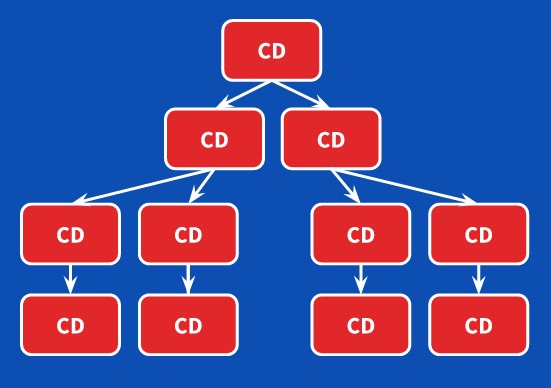
\includegraphics[width=0.7\linewidth]{kapitel3/cd-tree.jpg}
 \caption{Change Detection Flow}\cite{changedetection-explained}
\end{figure}

\newpage
\section{Ionic}

Im nachfolgenden soll die Relevanz des Frameworks Ionic 2 bezüglich des Projekts \projectname{} evaluiert werden.

\subsection{Einführung}

Ionic 2 ist ein Open Source \ac{SDK} für die Entwicklung mobiler Applikationen mithilfe von Angular 2 und Cordova.
Auf Basis von Webtechnologien wie HTML5, CSS3 und JavaScript können Apps für iOS, Android und Windowsphone
entwickelt werden. Diese werden als hybride Apps bezeichnet,
da sie eine Mischform zwischen Web-Apps und nativen Applikationen darstellen.
Eine hybride App ist zunächst eine Webanwendung, die einen Browser für ihre Ausführung benötigt.
Als Browser wird die native Webview der jeweiligen Platform verwendet,
beispielsweise Safari für iOS und Chrome für Android.
Mithilfe von Cordova Plugins kann auf das \ac{API} des Systems zugegriffen werden,
um Funktionalitäten wie beispielsweise GPS, Telefonbuch und Kamera zu verwenden \cite{ionic34:online}.

\subsection{Ionic Components}

\ac{UI} Elemente einer Ionic Anwendung werden mithilfe von Angular 2 Komponenten realisiert.
Dabei können diese, wie in einer Angular 2 App, anhand ihres HTML Selektors wiederverwendet werden.
Komponenten können dabei wiederum verschachtelt werden, so dass ein Komponentenbaum entsteht.

Das Ionic \ac{SDK} stellt Entwicklern eine ganze Reihe an vorgefertigten Komponenten zur Verfügung,
welche native Standardelemente der jeweiligen Plattform abdecken. Beispiele dafür sind Buttons, Listen, Tabs oder ActionSheets.
Interessant dabei ist, dass die Optik der Komponente dabei dem \ac{CI} der Plattform entspricht \cite{ionic99:online}.

\subsection{Theming}
Theming wird in einer Ionic Anwendung durch \ac{CSS} realisiert.
Styles werden entweder in eine Komponente gekapselt oder global definiert.
Globale Stile können dabei plattformspezifisch oder plattformunabhängig definiert werden.
So befinden sich in einer klassischen Ionic 2 App individuelle Styles für iOS, Android und Windowsphone.
Dadurch kann das umzusetzende \ac{CI} flexibel getreu dem Standard der Plattform entwickelt werden.
Soll eine Anwendung bezüglich Optik für jede Plattform identisch sein,
können plattformunabhängige, globale Stile definiert werden \cite{ionic73:online}.


\subsection{Ionic Native}

Ionic Native ist ein Wrapper für Cordova Module in JavaScript und Typescript.
In der Vorgängerversion des \ac{SDK} wurden Cordova Plugins installiert und als globale Singletons registriert.
Beispielsweise war es möglich, aus jedem Kontext der Applikation heraus ``navigator.camera.getPicture(onSuccess, onFail)'' aufzurufen.
Ionic Native hingegen erlaubt Entwicklern Module selektiv zu importieren, wodurch diverse Vorteile entstehen.
Globale Cordova Objekte werden vermieden, wodurch Code deutlich strukturierter und verständlicher wird.
Zudem werden Callbacks der Cordova Plugins mit Ionic Native in Promises oder Observables verpackt.
Dadurch entsteht ein einheitliches Interface im Stil von Angular 2 für die Nutzung dieser Module,
wodurch deren asynchrone Events bequemer observiert werden können.

Des Weiteren ist in Ionic Native eine Schicht für Fehlerbehandlung implementiert.
Ist ein Cordova Modul nicht installiert, oder wird es falsch verwendet,
generiert Ionic Native Fehler und Warnungen, die für Entwickler unabdingbar sind.
In der Vorgängerversion des Ionic \ac{SDK} konnten Fehler, die durch falsche Verwendung von
Cordova Modulen aufgetreten sind, meist nur durch ausprobieren oder Debugging des nativen Codes identifiziert werden
\cite{ionic55:online}.
Listing \ref{ionicnative} zeigt eine beispielhafte Implementierung der Kamera und GPS Schnittstellen mithilfe von Ionic-Native.

\vspace{0.3cm}
\lstinputlisting[language=JavaScript,label=ionicnative,caption=Ionic Native Beispiel \cite{ionic55:online}]{kapitel3/ionic-native-example.ts}


\subsection{Ökosystem Ionic}

``More than code. Ionic is an ecosystem. You'll find a suite of mobile development tools and resources at your disposal that make
Ionic the complete mobile dev package. It's the best way to build apps.'' \cite{Ionic20:online}
\vspace{0.5cm}

\paragraph{Ionic \ac{CLI}}
Die Ionic \ac{CLI} vereinfacht den Umgang mit Ionic Projekten erheblich. Zunächst können individuelle
Startertemplates anhand diverser Parameter generiert werden.
Das Framework erzeugt dabei voll funktionstüchtige Applikationen, die den Einstieg in das Framework erleichtern sollen.
\emph{Sidemenu} und \emph{Tabmenu} sind Beispiele für Templates, welche in Typescript oder JavaScript generiert werden können.
Darüber hinaus lassen sich Applikationen mithilfe der \ac{CLI} auf den Zielplattformen compilieren und auf angeschlossenen Geräten ausführen.

\paragraph{Ionic Creator}
ist ein Prototyping Tool, mit welchem Oberflächen statt
mit HTML und CSS per Mausklick kreiert werden können.
Dabei stehen von Beginn an eine Vielzahl von vorgefertigten Ionic Komponenten wie Buttons,
Label und Eingabefelder zur Verfügung.
Diese werden per Drag and Drop eingefügt und positioniert. Der Prototyp lässt sich jederzeit
als \ac{APK} oder \ac{IPA} für Dritte exportieren oder kann auf einem angeschlossenen Gerät gestartet werden.

\paragraph{Ionic Lab}
ist eine visuelle Oberfläche zur Bedienung der Ionic \ac{CLI}.
Buildvorgang, Testing und Deployment soll mithilfe der Desktop App für Mac, Windows, und
Linux speziell in Teams deutlich vereinfacht werden. \cite{Ionic75:online}

\subsubsection{Ionic Platform}

Ionic Platform ist eine Cloud, sowie eine Sammlung von Diensten für die Entwicklung,
Veröffentlichung und Skalierung von mobilen Apps. Zum Beispiel bietet Ionic Platform einen zentralen Dienst für die Nutzerverwaltung innerhalb einer App.
Nutzer können sich dabei klassisch per Mail oder per single sign on über
Facebook, Google und Twitter registrieren und sind damit in der Applikation authentifiziert.
Zudem können registrierte Nutzer zentral in einer Weboberfläche verwaltet und gegebenenfalls mit Push Nachrichten adressiert werden.
Diese können dabei an alle Nutzer, oder ein definiertes Segment gerichtet werden.
Hierzu ist kein Server mit implementiertem \ac{APN} oder \ac{GCM} System von Nöten, das Push System von Ionic deckt diese
Funktionalität bereits vollständig ab.

Zusätzlich kann die Cloud für das zentrale Deployment aller Zielplatformen genutzt werden.
Interessant hierbei ist, dass iOS Apps generiert werden können, auch wenn
keine macOS Umgebung zur Verfügung steht, da der Buildprozess in der Ionic Cloud stattfindet.
Ein App Update muss nicht zwingend über den Appstore der Plattform geschehen,
da Änderungen, die sich nur auf den Webinhalt der App (also HTML, CSS und JS) beziehen,
beim Appstart aus der Cloud geladen werden können.
Dies ermöglicht es Apps in Echtzeit zu deployen und Appstore Review Zyklen zu vermeiden.


\section{Electron}
\subsection{Allgemein}

Durch die stetige Entwicklung von Webbrowsern und Apps für Mobilgeräten haben Desktop Applikationen in den letzten Jahren immer mehr an Bedeutung verloren.
Dennoch bieten sie gegenüber Anwendungen, die nur in Browsern ausgeführt werden, einige Vorteile.
Desktop Anwendungen befinden sich im Dock beziehungsweise im Startmenü des Betriebssystems oder sind womöglich im Autostart referenziert.
Dadurch wirken sie präsenter, sind schneller zu erreichen und können selbst im minimierten Zustand noch Code ausführen.
Sie sind nicht durch Browser limitiert und können APIs der Betriebssysteme nutzen \cite{Build58:online}.

Electron ist ein Framework zur Entwicklung nativer Desktop Anwendungen, ebenfalls basierend auf Webtechnologien.
Atom, Visual Studio Code, Whatsapp und Slack sind erfolgreiche Beispiele für Anwendungen, die mithilfe von Electron
entwickelt wurden.
Der Fokus soll bei der Entwicklung auf die eigentliche Geschäftslogik der Anwendung und nicht auf plattformspezifische
``hard parts'' der nativen Desktop Entwicklung gerichtet werden \cite{Elect57:online}.

\vspace{0.3cm}
``If you can build a website, you can build a desktop app. Electron is a framework for creating native applications
with web technologies like JavaScript, HTML, and CSS. It takes care of the hard parts so you can focus on the core of
your application.''
\cite{Elect57:online}

\subsection{Funktionsweise}
\label{sec:functionsweise}


Wie in Abbildung \ref{fig:electronprozess} dargestellt, werden beim Start einer
Electron Anwendung verschiedenen Prozesskontexte gestartet.
Zunächst startet der Hauptprozess (main Process), in welchem grundlegende Konfigurationen vorgenommen werden können.
Die Besonderheit dieses Kontextes ist die Verfügbarkeit von Node.js.
Mit Node.js erhält man Zugriff auf Schnittstellen des Betriebssystems um beispielsweise Dateien lesen oder schreiben zu können.
Ferner wäre es im Hauptprozess möglich einen API oder Websocket Server zu starten.

Der Hauptprozess instanziiert den Kontext der Webview, in Abbildung \ref{fig:electronprozess} wird dieser als render process bezeichnet.
Dieser beinhaltet eine Browserumgebung, welcher die \ac{UI} der Anwendung in einem für den Nutzer sichtbaren Fenster darstellt.
Die Webinhalte werden dabei mit Chromium, der quellofenen Basis von Google Chrome, gerendert \cite{Build58:online}.

\begin{figure}[htbp]
 \centering
 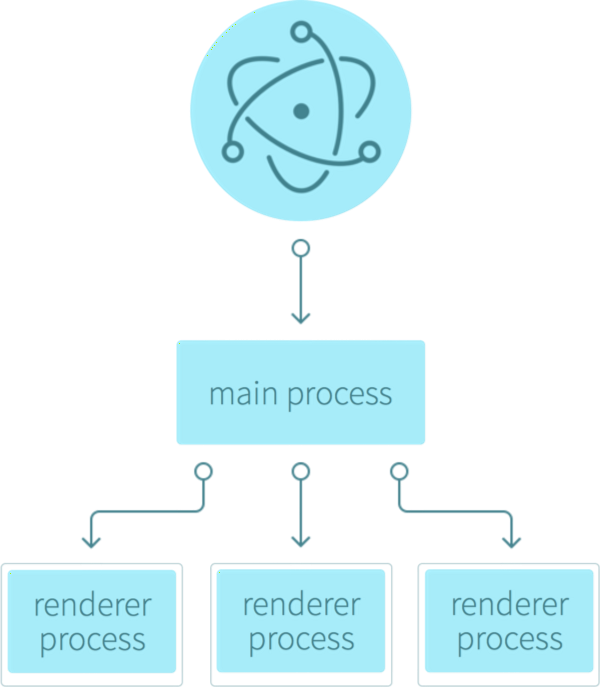
\includegraphics[width=0.4\linewidth]{kapitel3/electron-context.png}
 \caption{Electron Prozesse \cite{Build58:online}}
\label{fig:electronprozess}
\end{figure}


\subsection{Kommunikation}
\label{sec:Kommunikation}

Da Node.js nur im Hauptrozess von Electron genutzt werden kann, ist es erforderlich,
dass die verschiedenen Kontexte miteinander interagieren beziehungsweise kommunizieren können.
Dies kann, wie bereits in \ref{sec:functionsweise} Funktionsweise angesprochen,
mithilfe eines zentralen API Servers oder Websockets stattfinden.
Die Electron API bietet eine weitere Möglichkeit für eine Interprozesskommunikation.
Dem Main- und Render Prozess wird jeweils eine IPC Event Emitter Instanz zur Verfügung gestellt,
über welche asynchrone Events gesendet und empfangen werden können.

\section{\ac{NPM}}

\ac{NPM} ist ein Package Manager für Node.js und JavaScript mit insgesamt mehr als 300.000 verschiedenen Paketen und
4.939.882.172 Paket Installationen im Juni 2016.
Open Source Pakete können kostenfrei veröffentlicht werden.
Für die Verwaltung von Closed Source Paketen wird ein Preismodell ab 7\$ pro Monat angeboten.
Dependencies des Projekts \projectname{}, also Pakete wie Angular, Ionic und Electron können vollständig
über \ac{NPM} geladen werden \cite{npm31:online}.

Ein \ac{NPM} Modul beinhaltet neben dem Programmcode eine Package.json Datei, in welcher relevante Metainformationen über das Modul selbst und den Autor gespeichert werden.
Zusätzlich können in der Package.json post-Installation Scripte referenziert werden um
beispielsweise eine Transpilierung von TypeScript zu JavaScript vornzunehmen, nachdem das Modul als Abhängigkeit installiert wurde.
Die Veröffentlichtung in der Registry und damit auf \emph{npmjs.com} sowie der Updatevorgang eines Moduls geschieht über die \ac{CLI} von \ac{NPM}.

\section{Gulp}

Gulp ist ein Build System zur Ablaufoptimierung und Automatisierung komplexer Softwareprodukte.
Das System basiert auf Node.js Streams, kann jedoch auch für Plattformen wie Java, PHP und .Net verwendet werden.
Automatisierungen werden mit Gulp in Form von Tasks implementiert,
welche typischerweise Dateien lesen, diese innerhalb von Streams verarbeiten und das Ergebis wiederum auf die
Festplatte schreiben \cite{gulpj46:online}.
Tasks können dabei manuell, oder über Filewatcher durch Dateiänderungen ausgelöst werden.
Anwendungsfälle für Gulp Tasks sind beispielweise Transpilierung von Typescript zu JavaScript Code oder
Automatisierung von Deployment Prozessen. Die \ac{NPM} Registry beinhaltet bereits über 14.000 Open Source Plugins,
mit denen die Grundfunktinalität von Gulp erweitert werden kann \cite{resul14:online}.
Gulp selbst wurde im Juni 2016 2.304.745 mal per NPM installiert \cite{gulp17:online}.

%!TEX root = ../thesis.tex

\chapter{Workflow Optimierung mit Gulp}


\section{Allgemein}
\section{Entwicklung der Komponenten}
\section{Verteilung der Komponenten}
\section{Produktion}
\section{Continuous Deployment für Updates der Desktop Applikation}



\listoffigures
\lstlistoflistings
\listoftables

\bibliographystyle{apalike}
\bibliography{citeulike}
\end{document}
